\section{Scenarios and Results}
In order to test the simulation framework, three different scenarios were created with unique design choices and characteristics. Each of them designed to represent a simplified real-world scenario with their own challenges and management implications. These scenarios represent three major types of fires: Extreme weather events, human-wildland interface conditions and complex coastal fire dynamics. Each of the scenarios have different parameter sets and environmental conditions to show the models ability to capture a diverse fire behaviors.

\subsection{Drought Firestorm Scenario}
The first scenario represents a very extreme fire weather conditions and intends to simulate the type of catastrophic fires that occur after a long period drought with very low level of moisture. These types of conditions are becoming more prevalent with the climate change, that we are experiencing right now. Furthermore this scenario serves as baseline for maximum fire potential and validates the model ability to handle a large number of fire events similar to California's recent Megafires or Australia's Black Summer fires.\newline
\newline
\textbf{Configuration}:
\begin{itemize}
	\item Map Type: Forest
	\item Wind strength: 0
	\item Moisture: 0
	\item Fuel Types: 6 distinct heterogeneous patches
	\item Multiple ignition points
\end{itemize}
\textbf{Key Parameters}:
\begin{itemize}
	\item \texttt{spread\_rate}: 0.08 (base velocity of particles)
	\item \texttt{ignition\_probability}: 0.15 (base probability for ignition)
	\item \texttt{particle\_generation\_rate}: 0.18
	\item \texttt{burnout\_rate}: 0.005 (Rate at which burning cells burnout)
\end{itemize}

\subsubsection{Spatial Analysis Results}
Figure~\ref{fig:spatial_df} shows the spatial analysis of the simulation, which reveals several patterns: \newline

\begin{figure}[H]
	\centering
	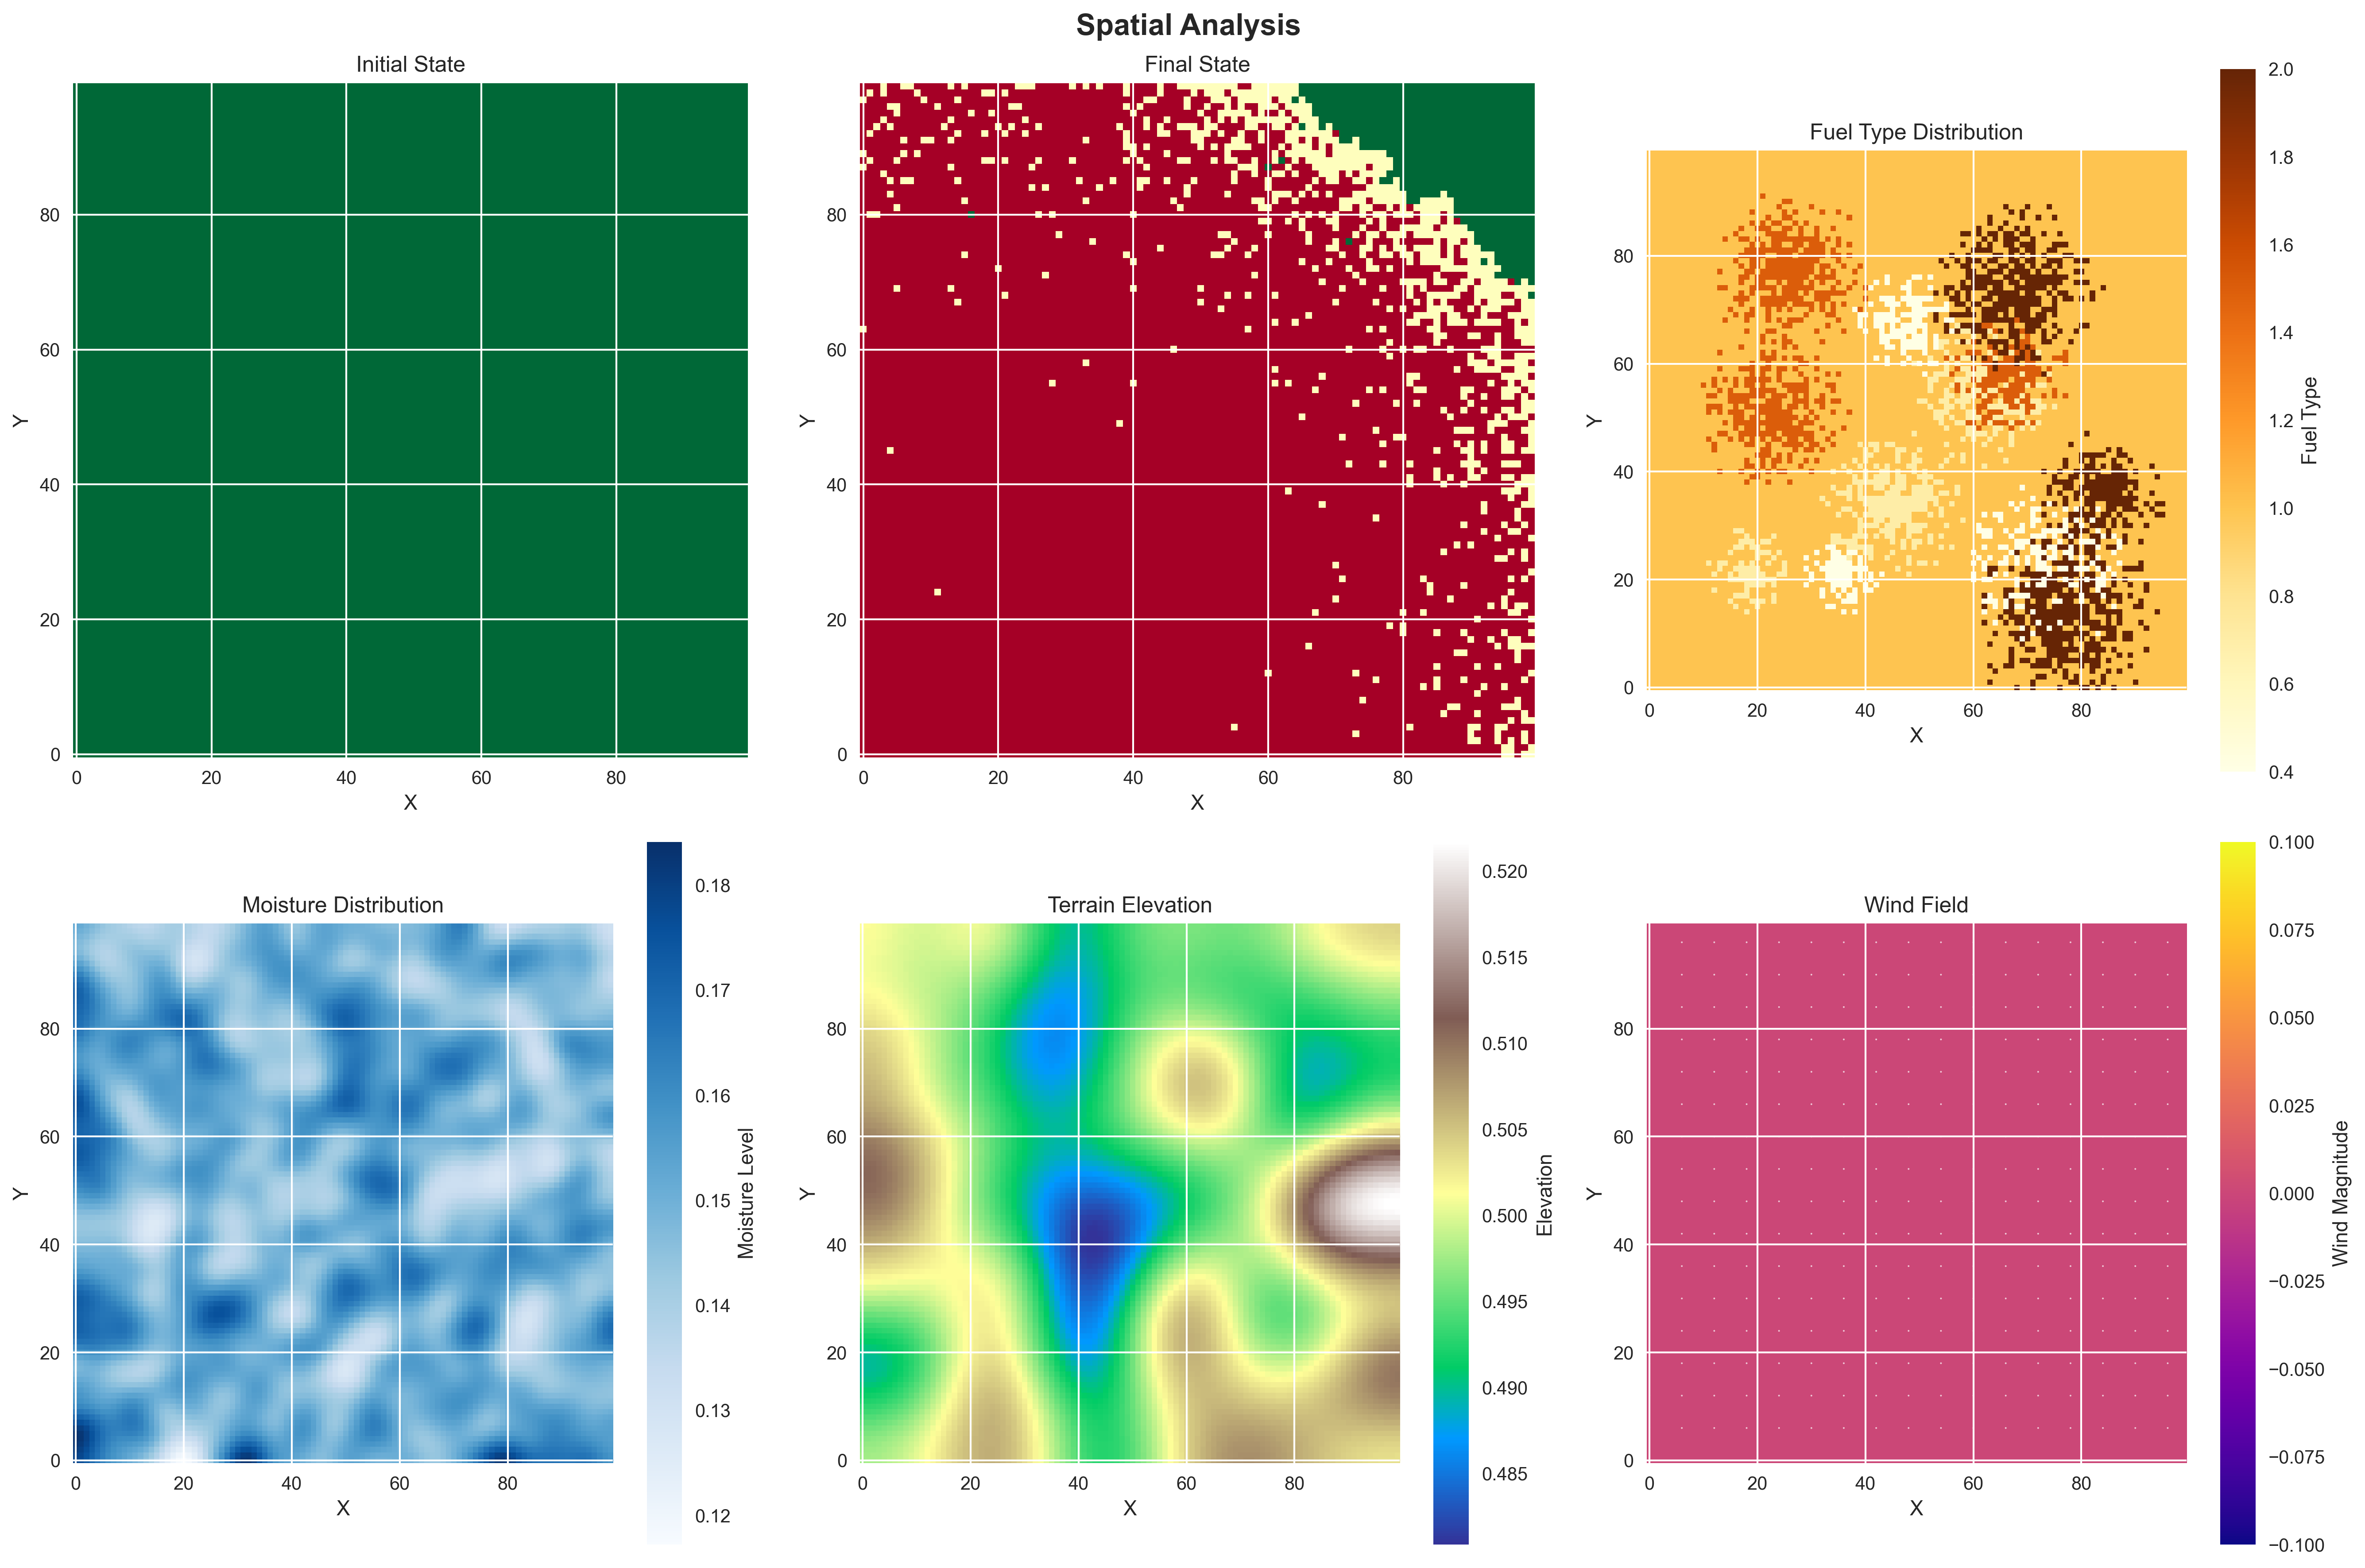
\includegraphics[width=\textwidth]{media/spatial_analysis_df.png}
	\caption{
		\textbf{Spatial Analysis - Drought Firestorm Scenario.} 
		Environmental conditions and fuel distribution for the drought firestorm simulation. Top row shows initial state (left) with uniform fuel distribution, final state (center) with extensive burned area coverage, and fuel type distribution (right) with heterogeneous patches ranging from grassland (light) to dry brush (dark). Bottom row displays moisture distribution (left) showing minimal moisture content, terrain elevation (center) with topographic variations, and wind field (right) showing on wind. 
	}
	\label{fig:spatial_df}
\end{figure}

\begin{figure}[H]
	\centering
	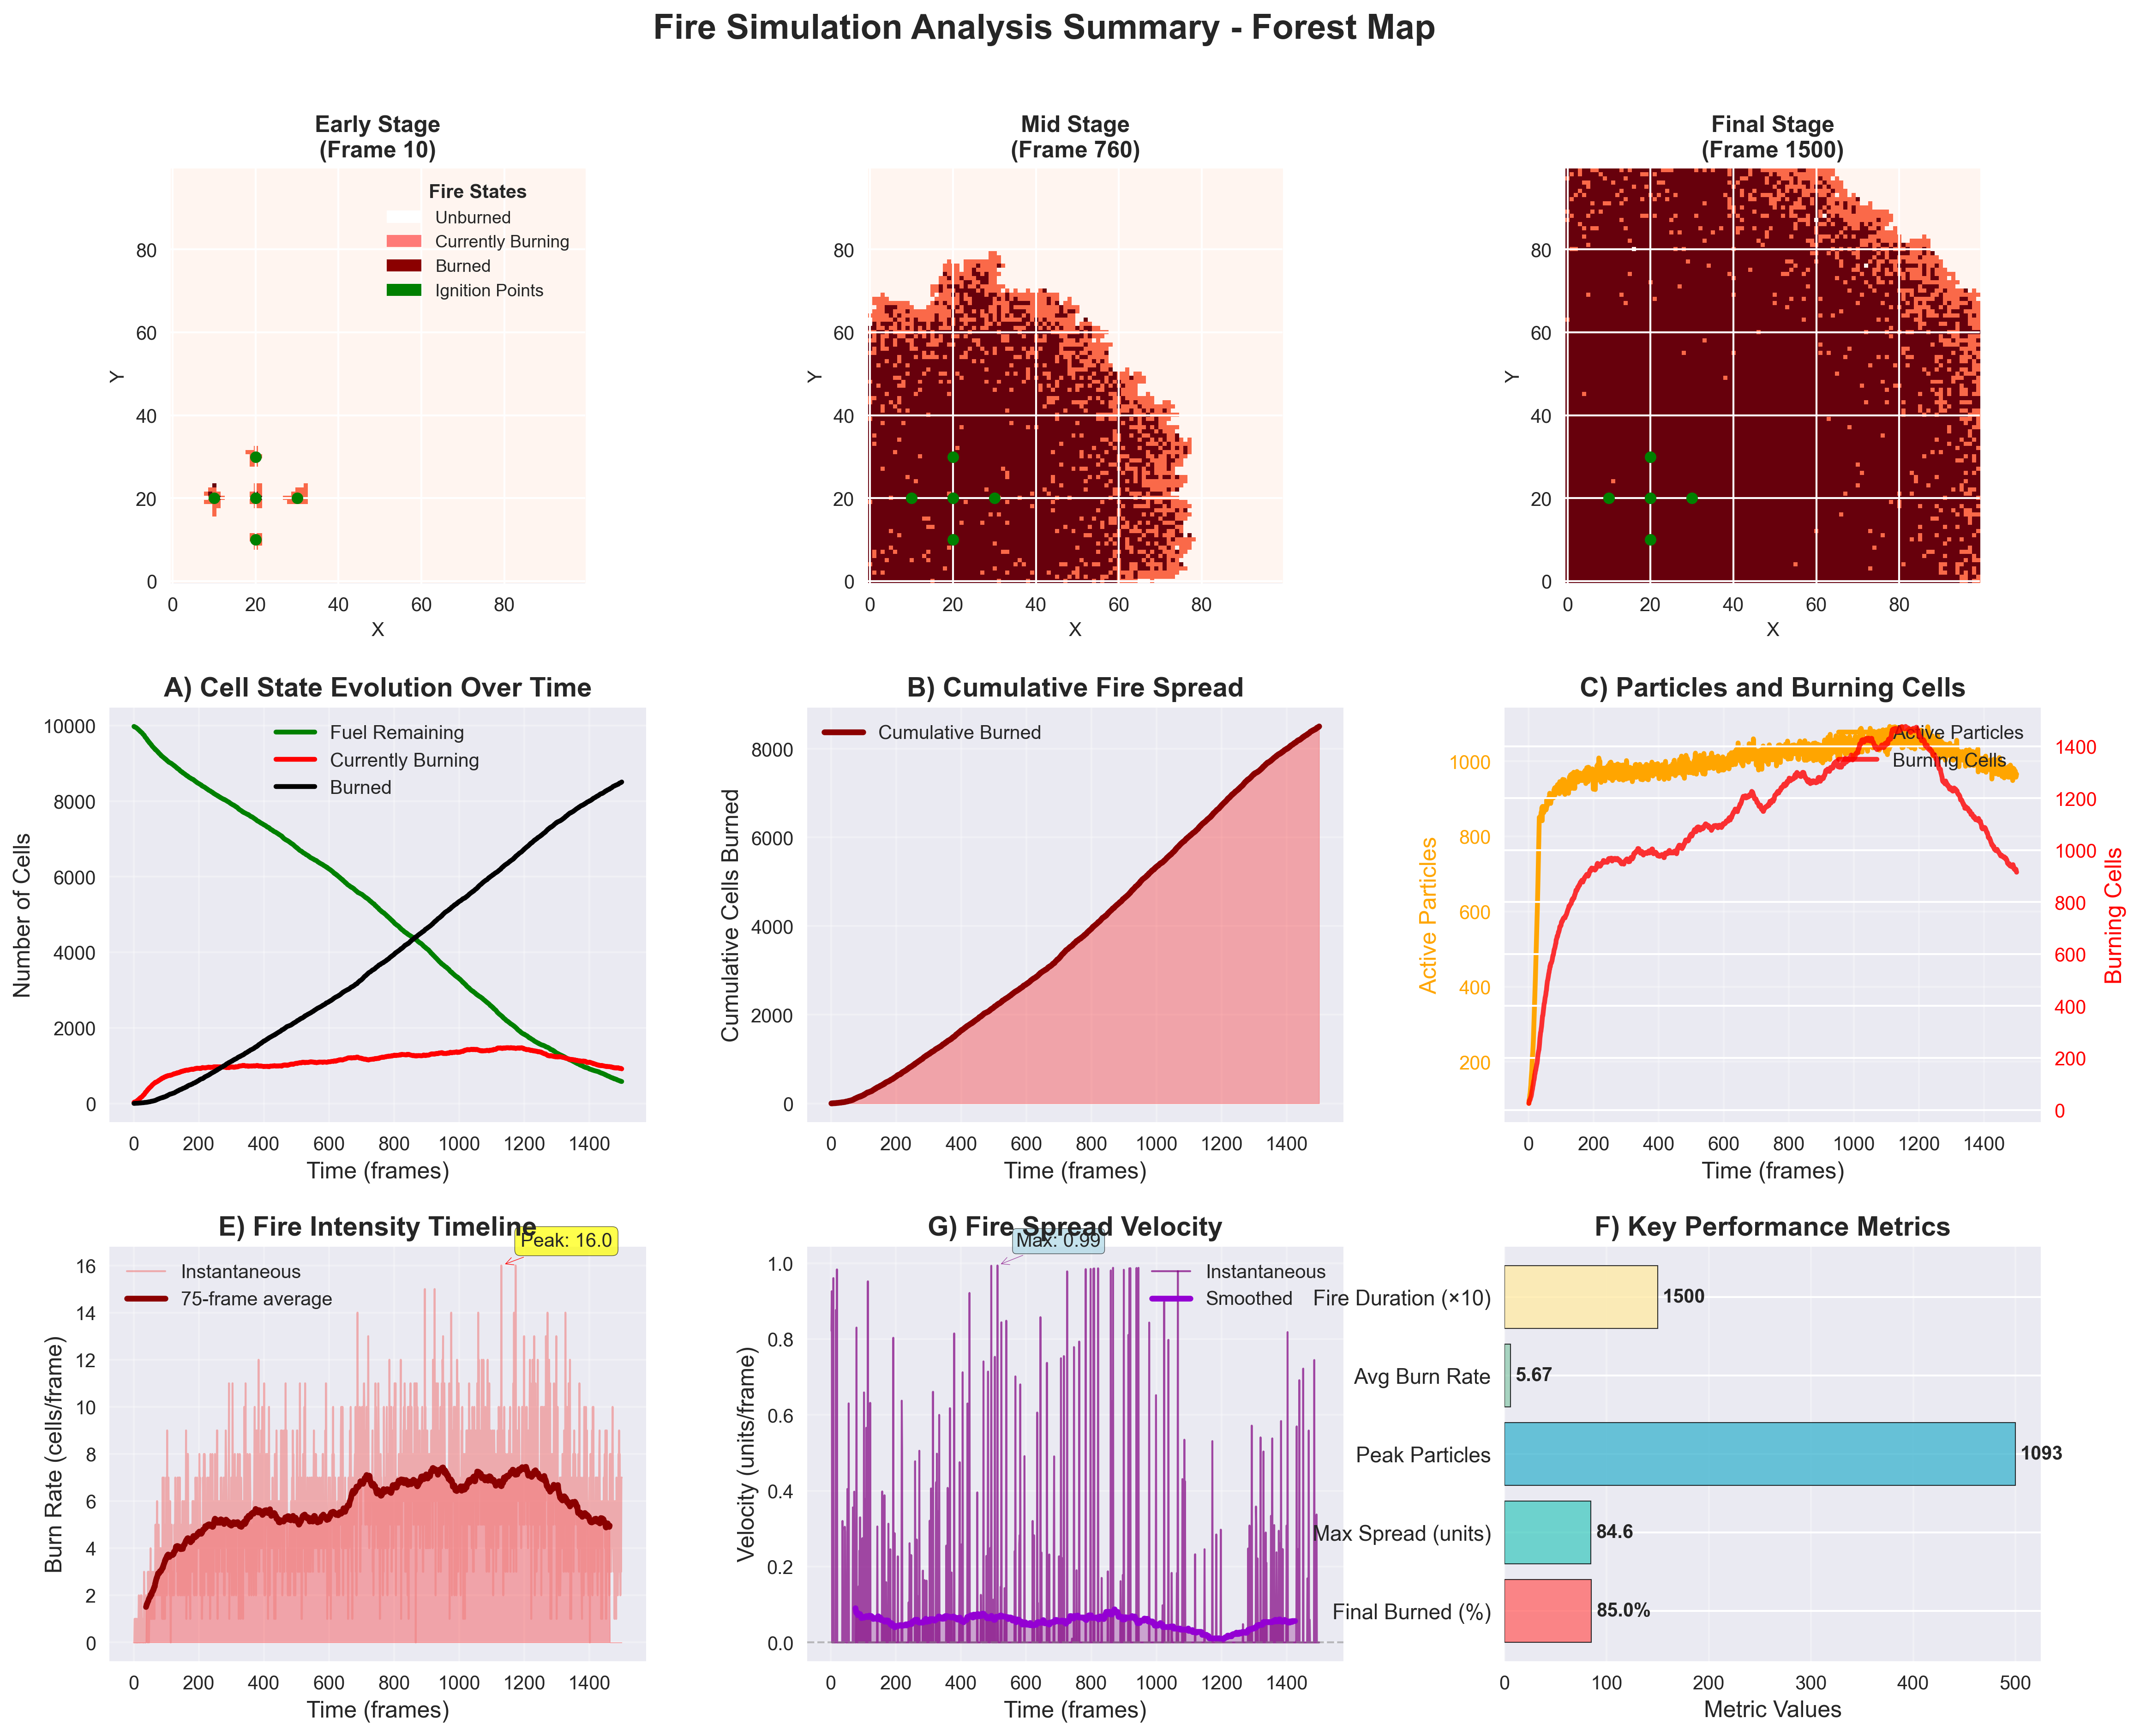
\includegraphics[width=\textwidth]{media/report_summary_df.png}
	\caption{
		\textbf{Fire Simulation Analysis Summary - Drought Firestorm.} 
		Comprehensive analysis of fire progression under extreme drought conditions. Top row shows fire evolution from early ignition (left) through mid-stage development (center) to final extensive coverage (right). Middle row presents cell state evolution over time (A), cumulative fire spread (B), and particle-burning cell dynamics (C). Bottom row displays fire intensity timeline (E), fire spread velocity (G), and key performance metrics (F) including 85.9\% final burned area and peak particle count of 1093.
	}
	\label{fig:res_df}
\end{figure}

\subsection{Wildland Urban Scenario}
\begin{figure}[H]
	\centering
	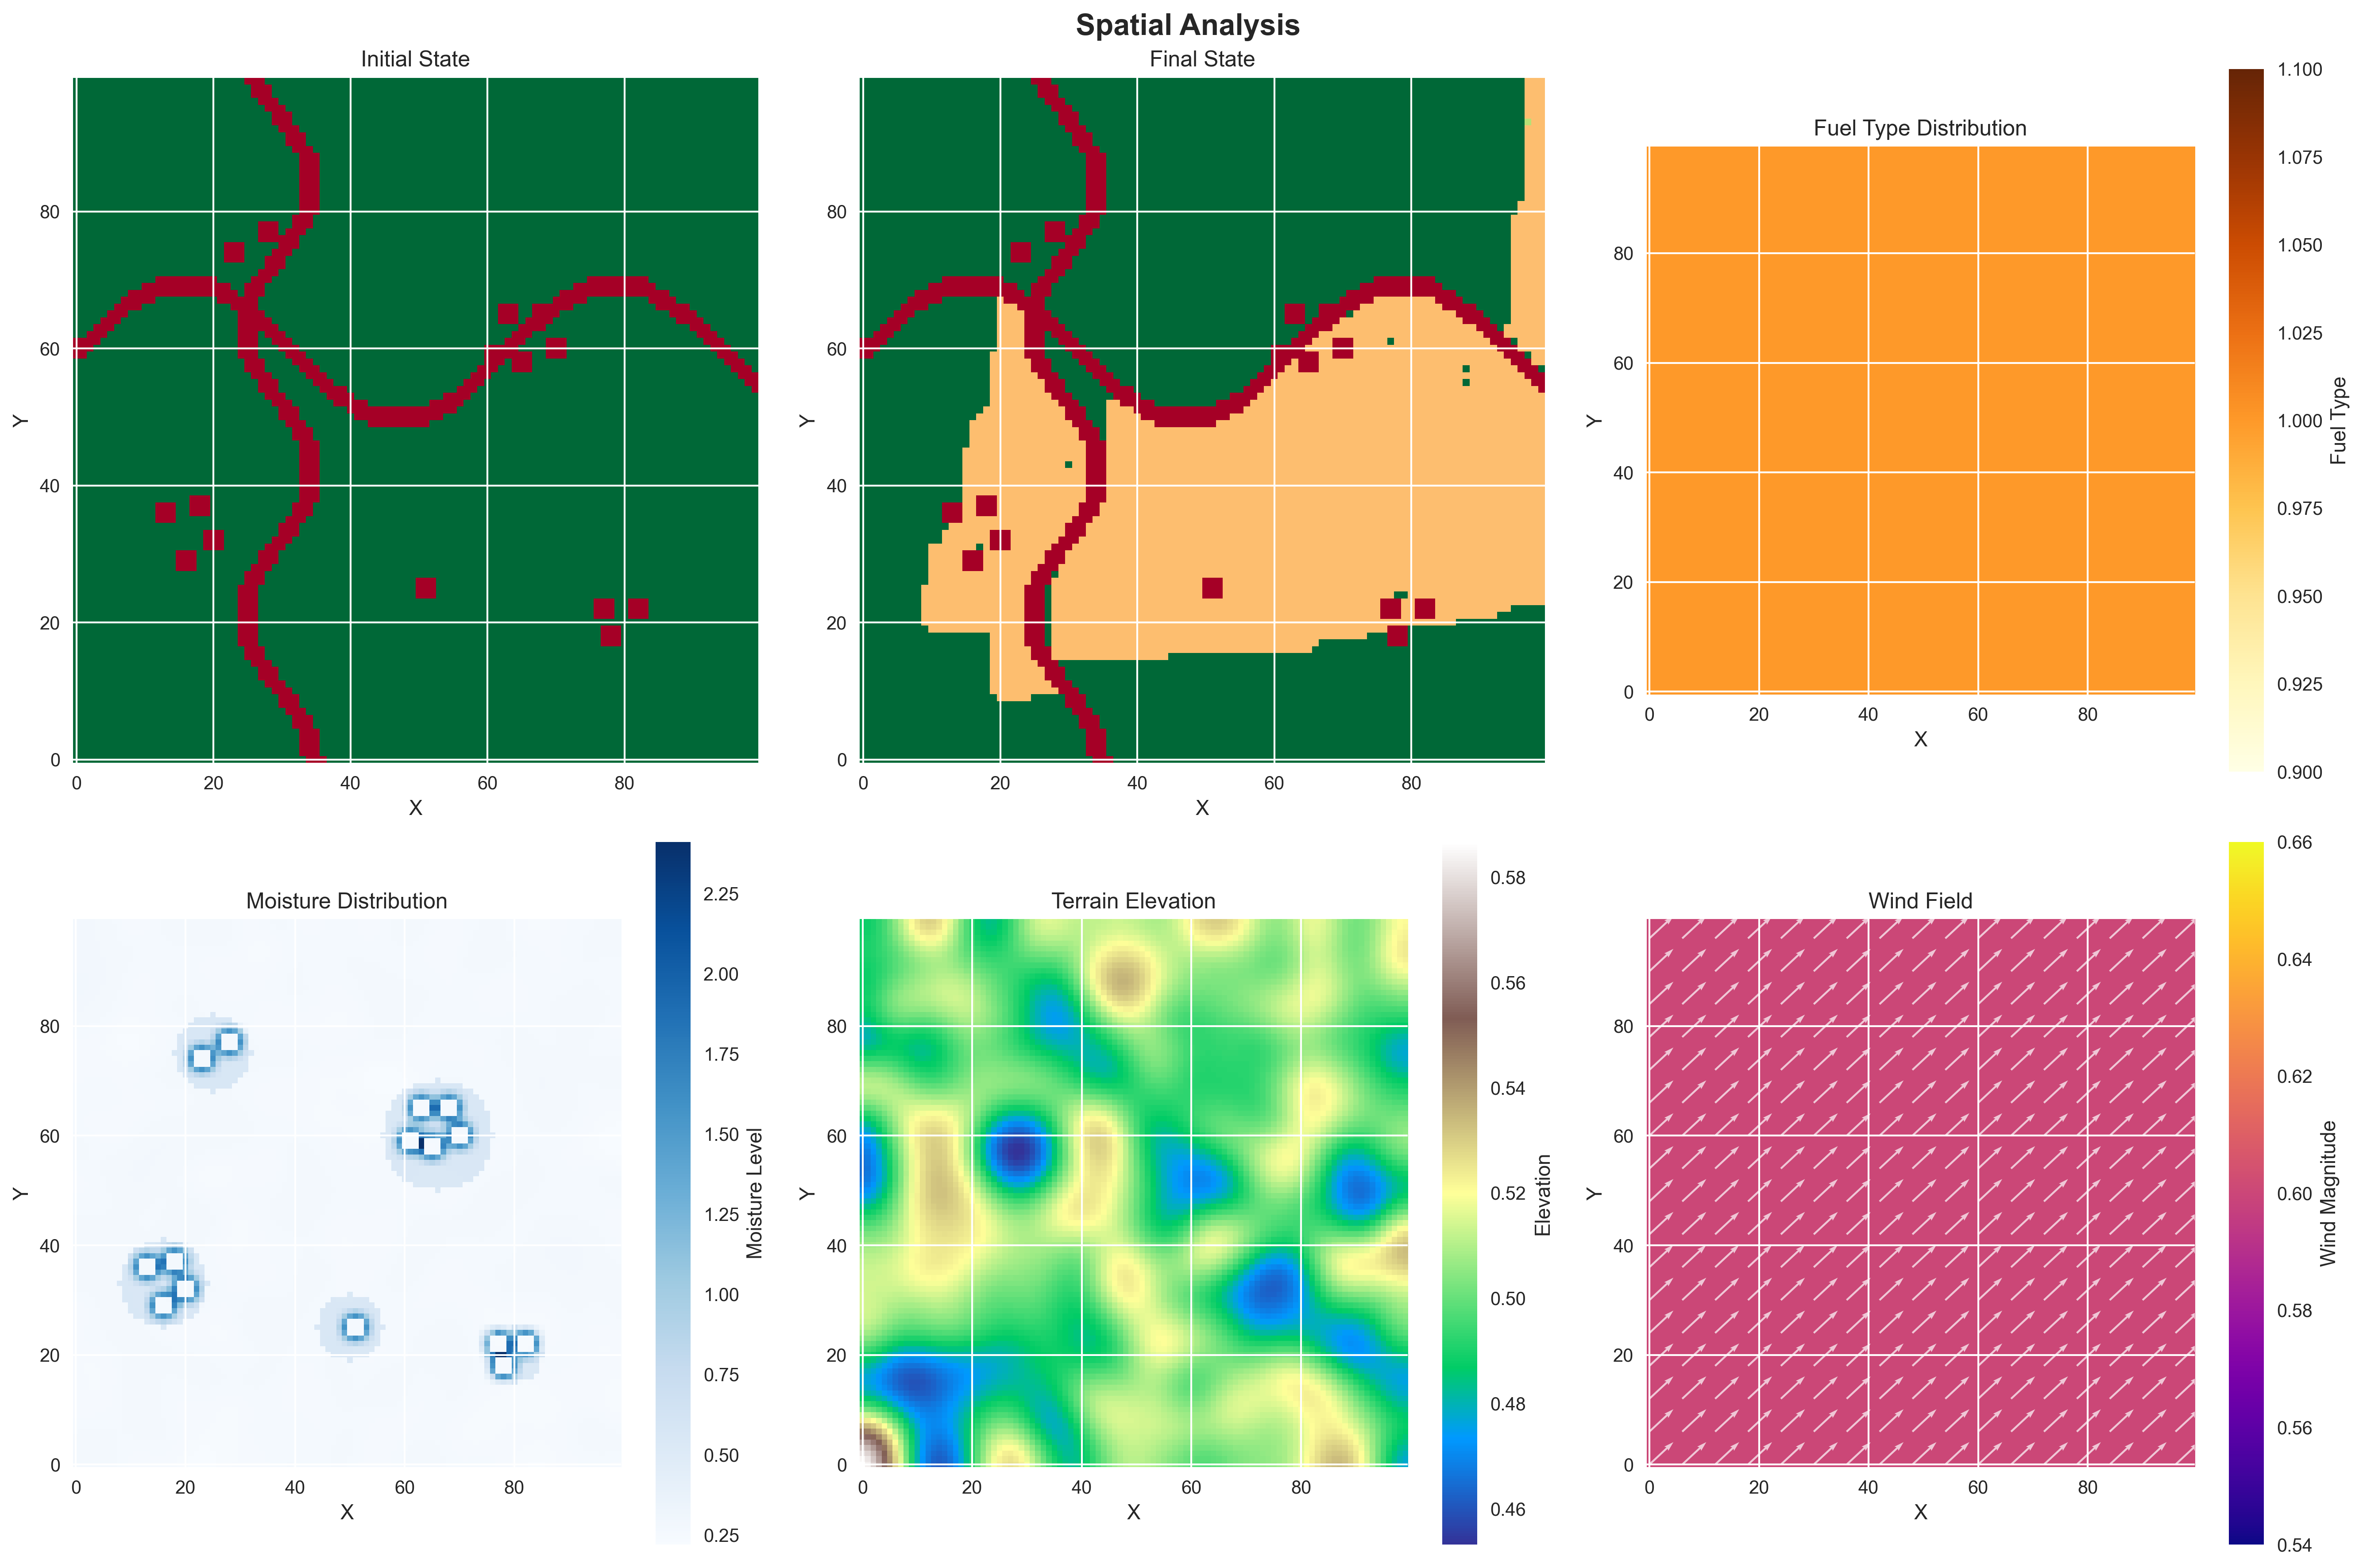
\includegraphics[width=\textwidth]{media/spatial_analysis_wui.png}
	\caption{
		\textbf{Spatial Analysis - Wildland Urban Interface Scenario.} 
		Environmental conditions for WUI fire simulation showing the interaction between natural fuels and residential development. Top row displays initial state (left) with scattered housing clusters and defensible space, final state (center) showing fire containment around structures, and fuel type distribution (right). Bottom row shows moisture distribution (left) with elevated moisture around structures, terrain elevation (center), and wind field (right) with moderate directional wind creating asymmetric fire spread potential.
	}
	\label{fig:spatial_wui}
\end{figure}

\begin{figure}[H]
	\centering
	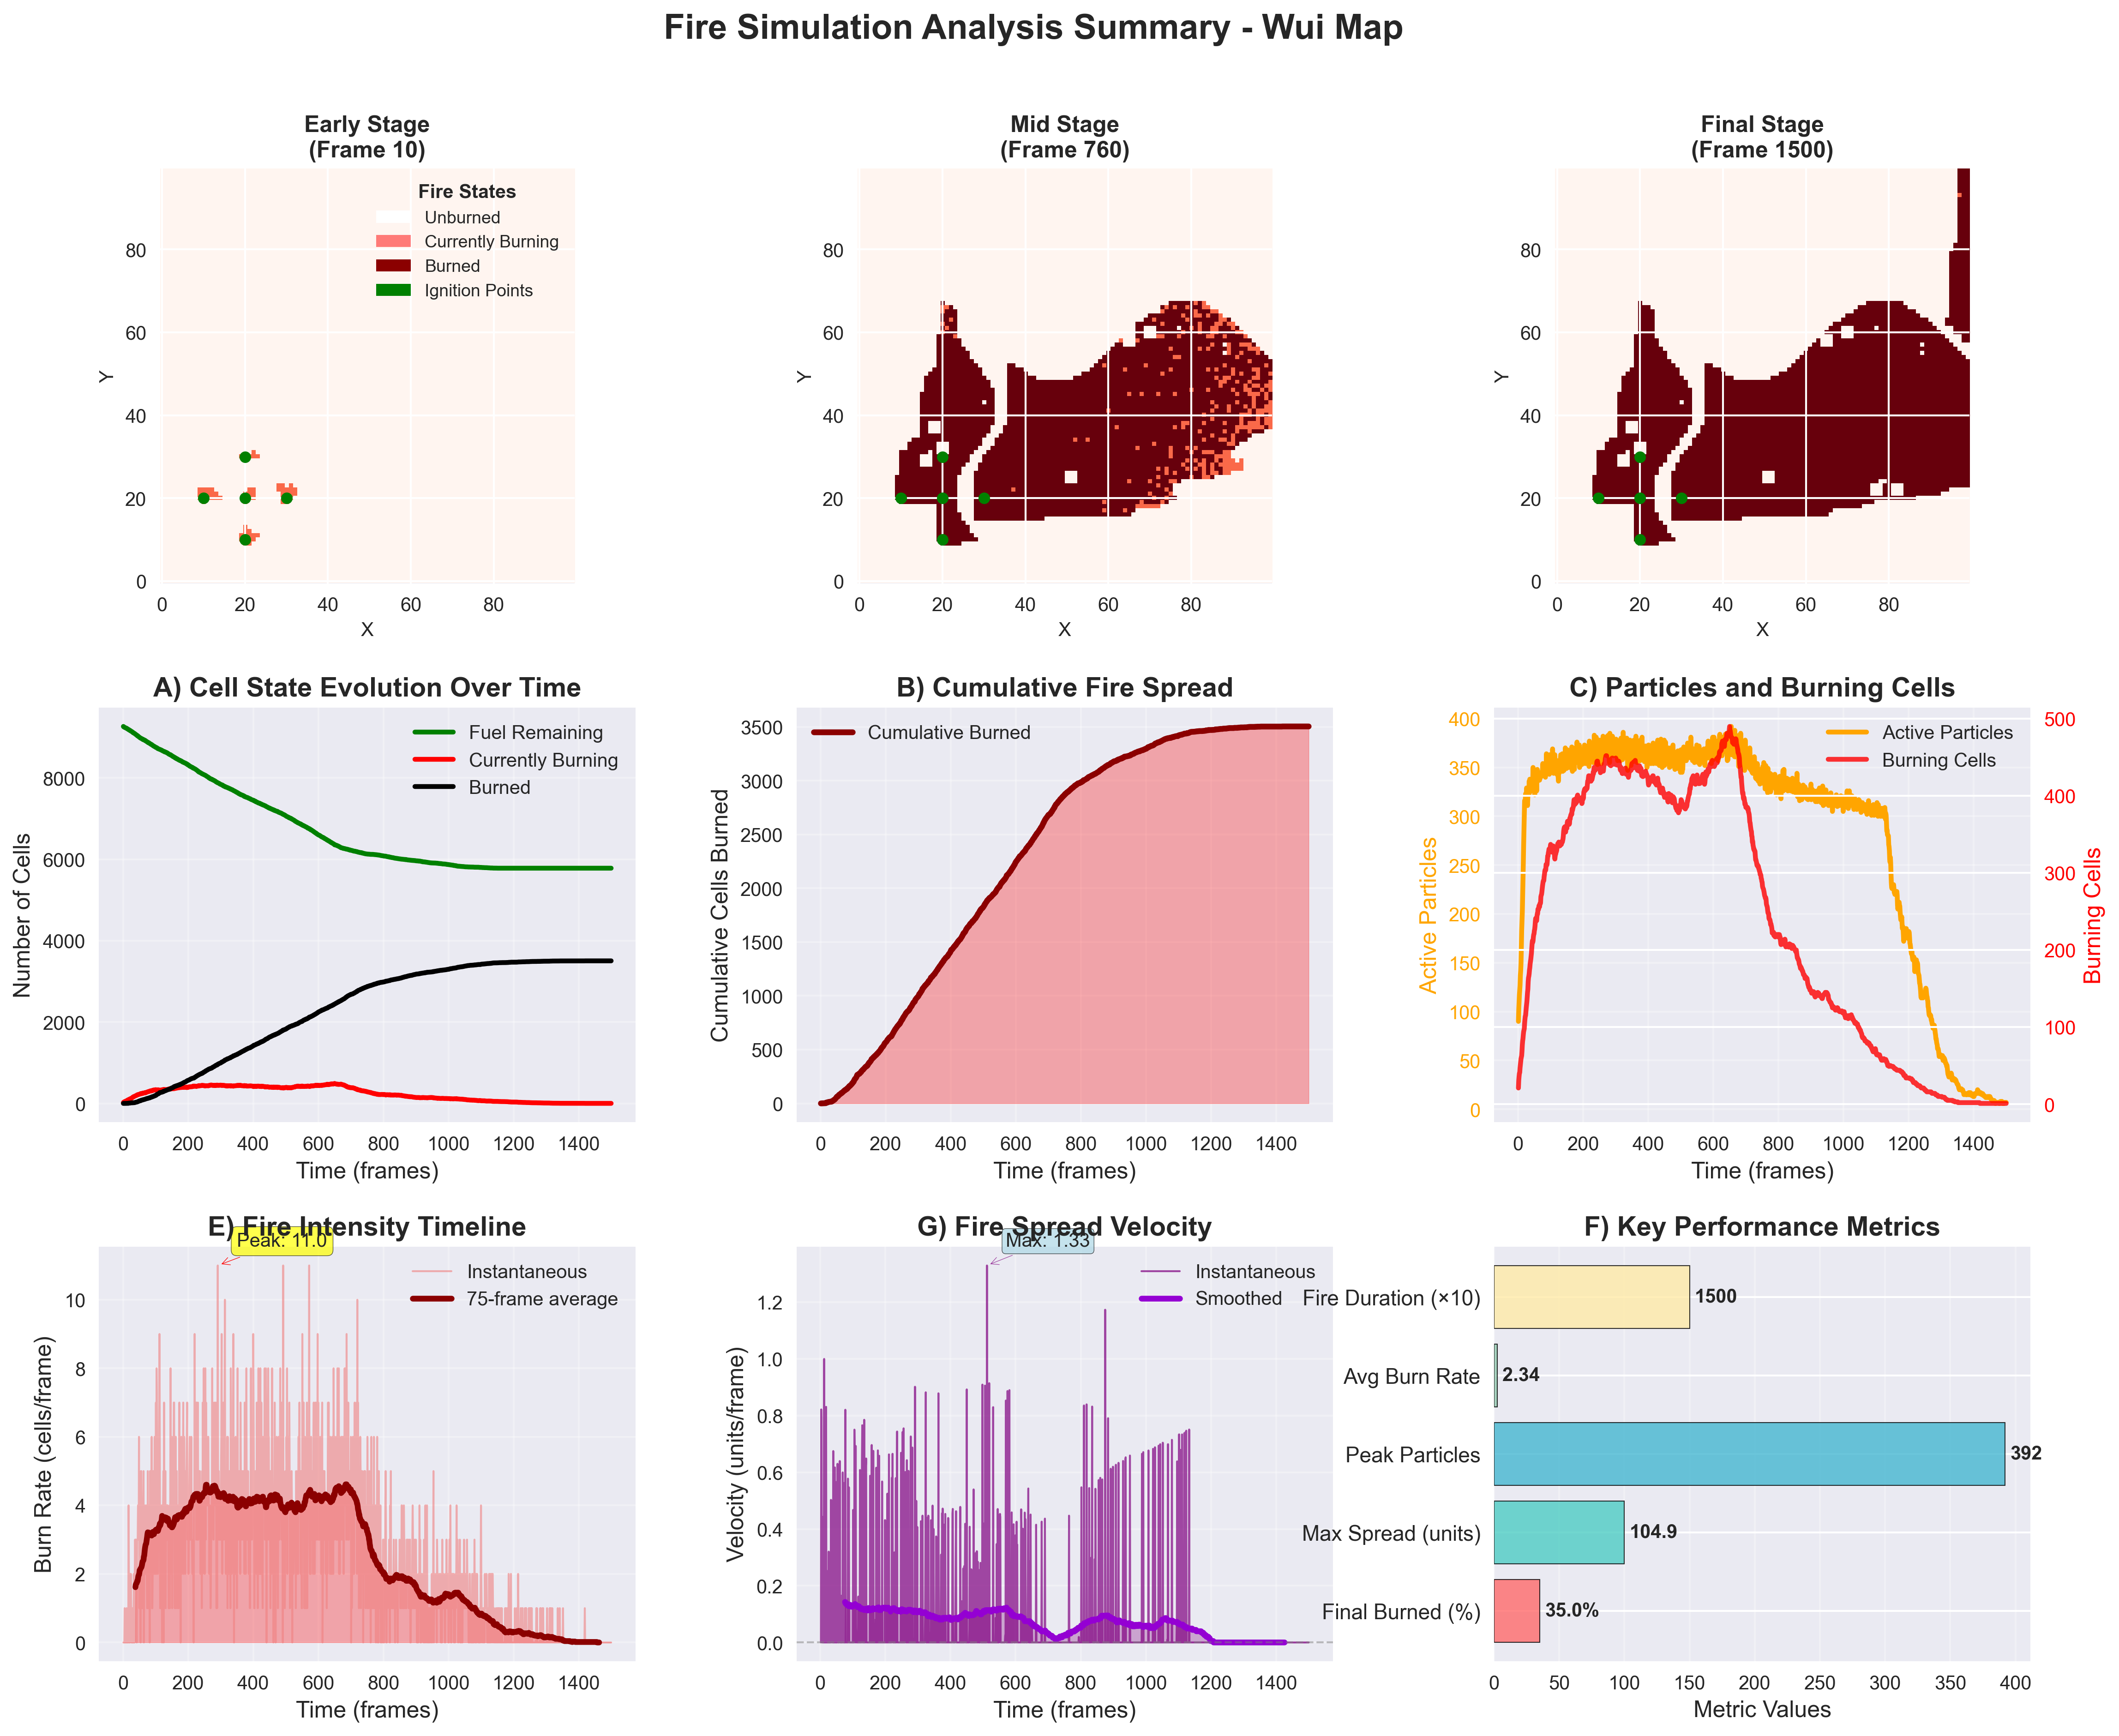
\includegraphics[width=\textwidth]{media/report_summary_wui.png}
	\caption{
		\textbf{Fire Simulation Analysis Summary - Wildland Urban Interface.} 
		Analysis of fire behavior in developed wildland areas demonstrating effective structure protection. Top row shows fire progression with early containment (left), mid-stage development around barriers (center), and final controlled burn area (right). Middle and bottom rows present temporal analysis showing reduced fire intensity compared to drought conditions, with 35.0\% final burned area and successful defensible space performance protecting all residential structures.
	}
	\label{fig:res_wui}
\end{figure}

\subsection{Coastal Scenario}
\begin{figure}[H]
	\centering
	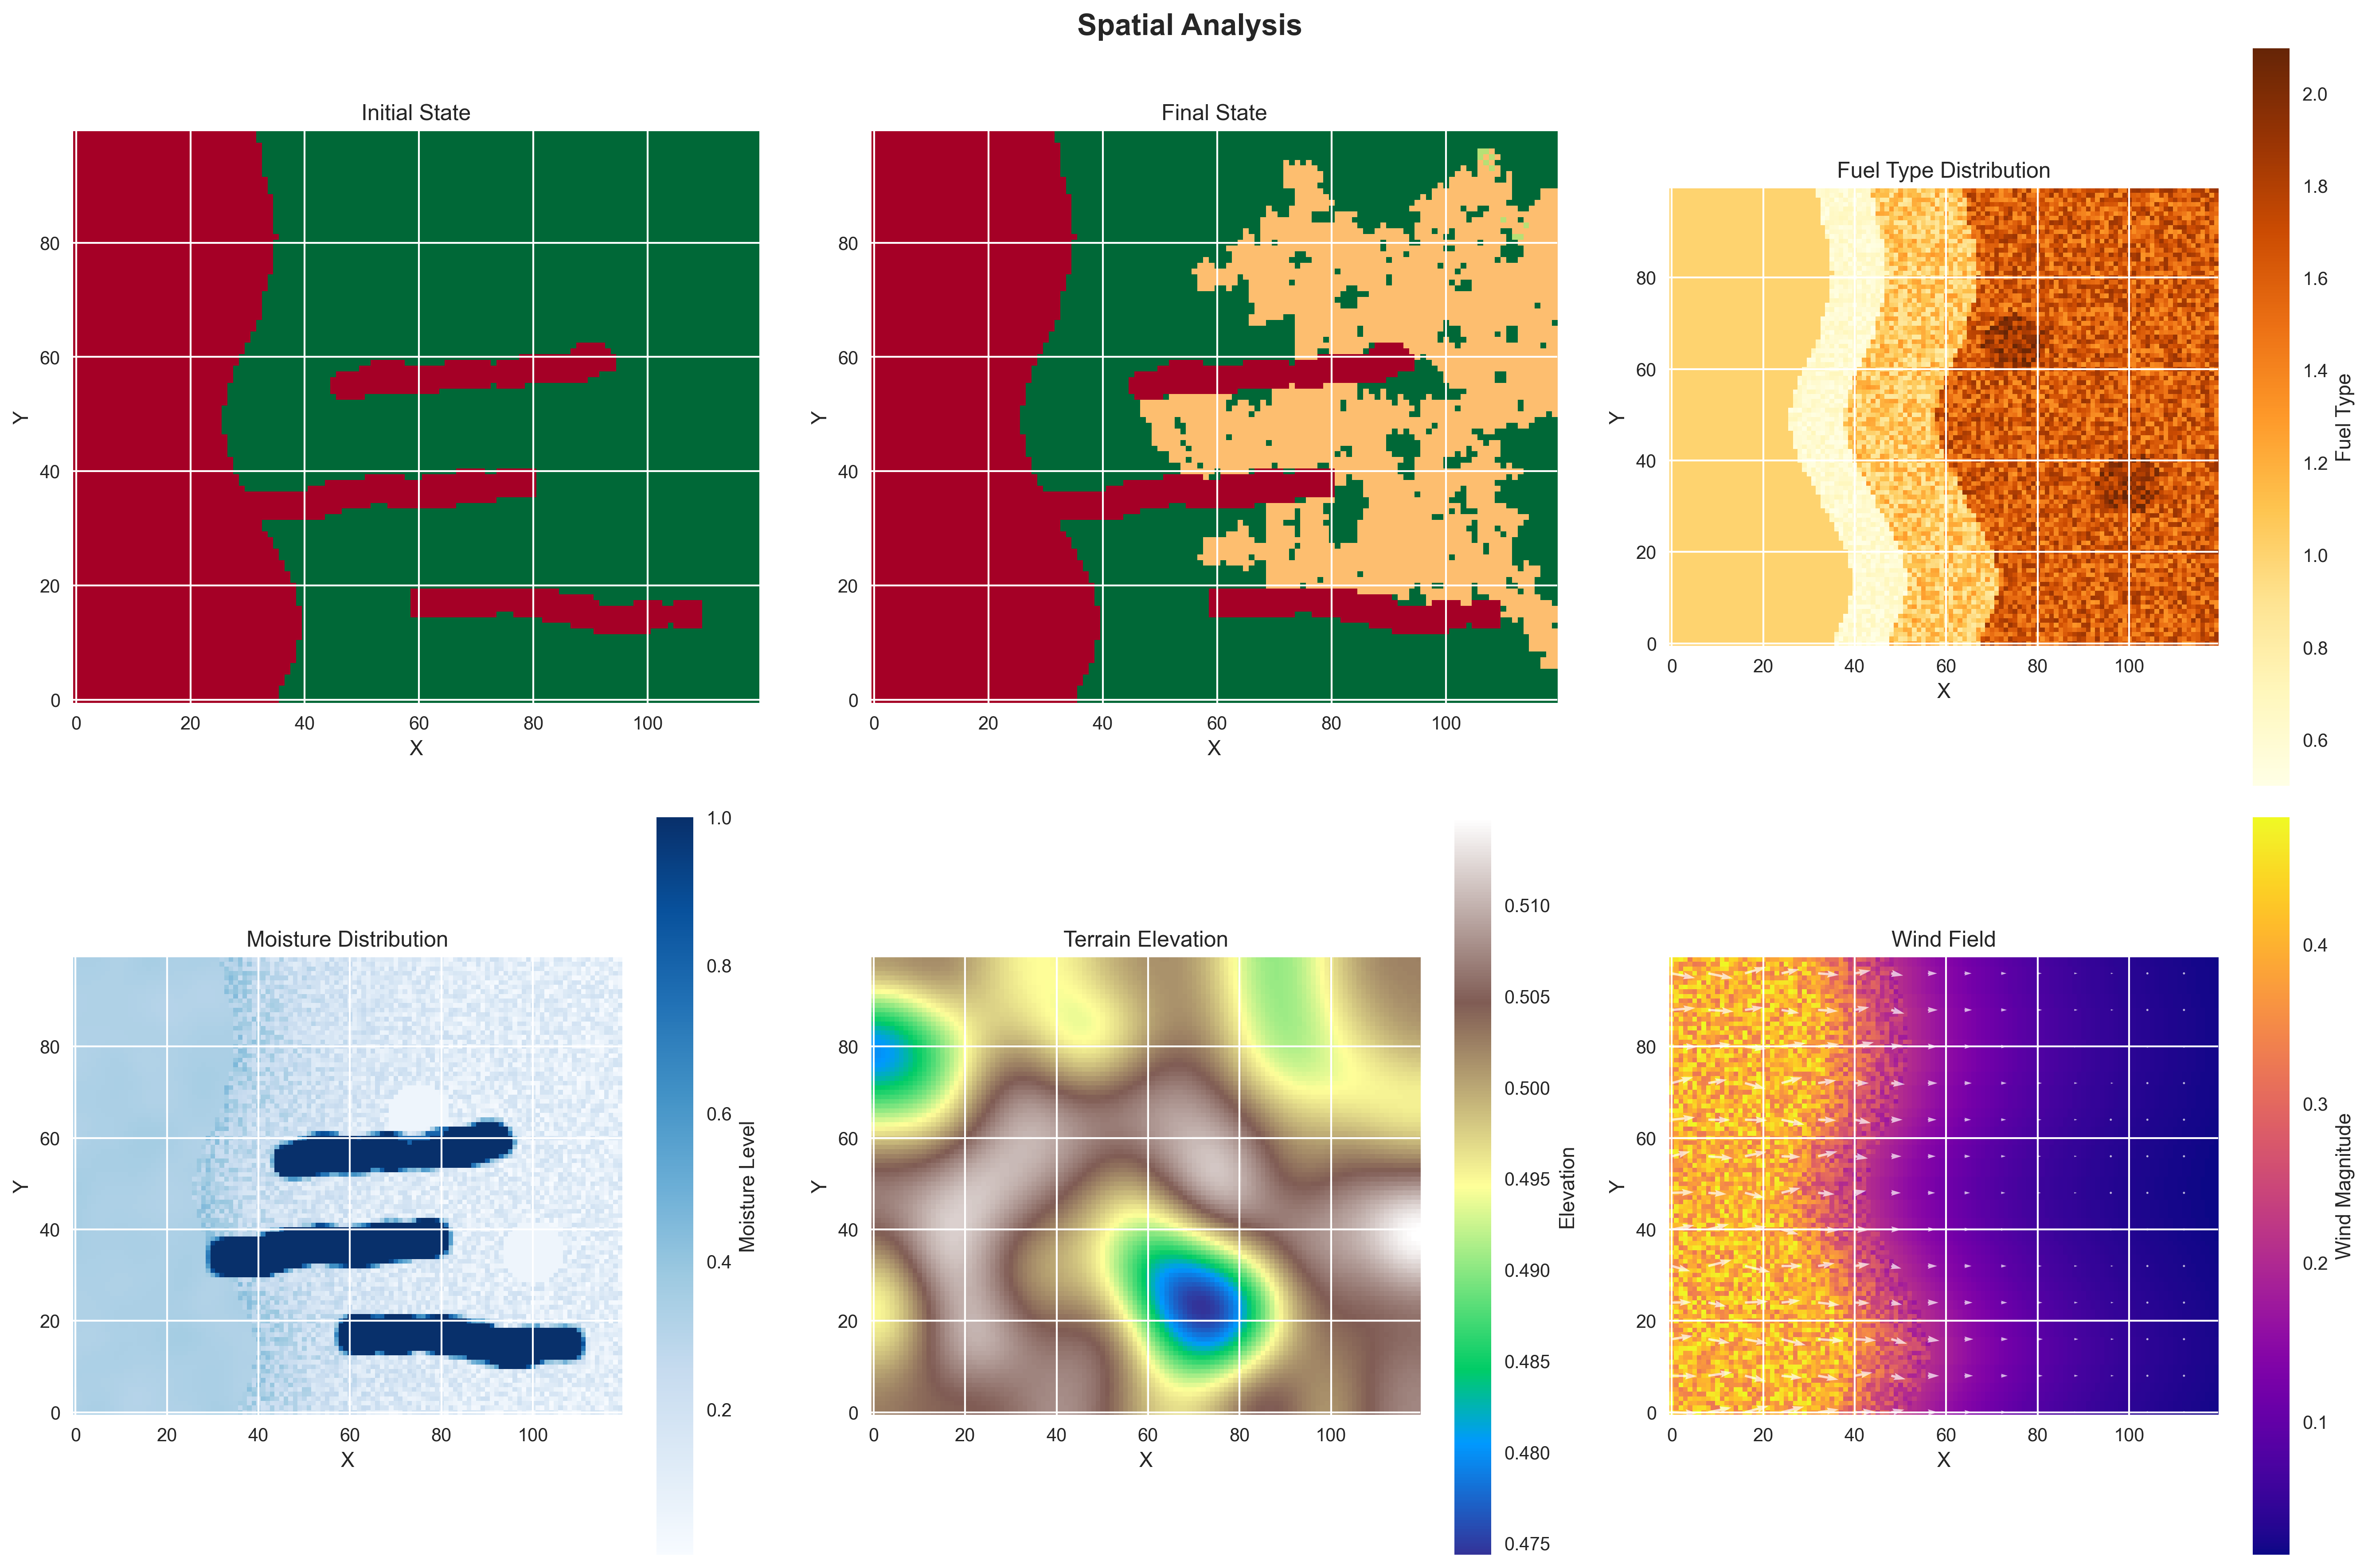
\includegraphics[width=\textwidth]{media/spatial_analysis_coast.png}
	\caption{
		\textbf{Spatial Analysis - Coastal Fire Scenario.} 
		Environmental conditions for coastal fire simulation featuring moisture gradients and strong offshore winds. Top row shows initial state (left) with coastline and natural barriers, final state (center) demonstrating inland fire penetration with coastal protection, and fuel type distribution (right) varying from coastal scrub to inland chaparral. Bottom row displays moisture distribution (left) with clear coastal-to-inland gradient, terrain elevation (center), and strong wind field (right) creating offshore wind patterns typical of extreme fire weather events.
	}
	\label{fig:spatial_coast}
\end{figure}

\begin{figure}[H]
	\centering
	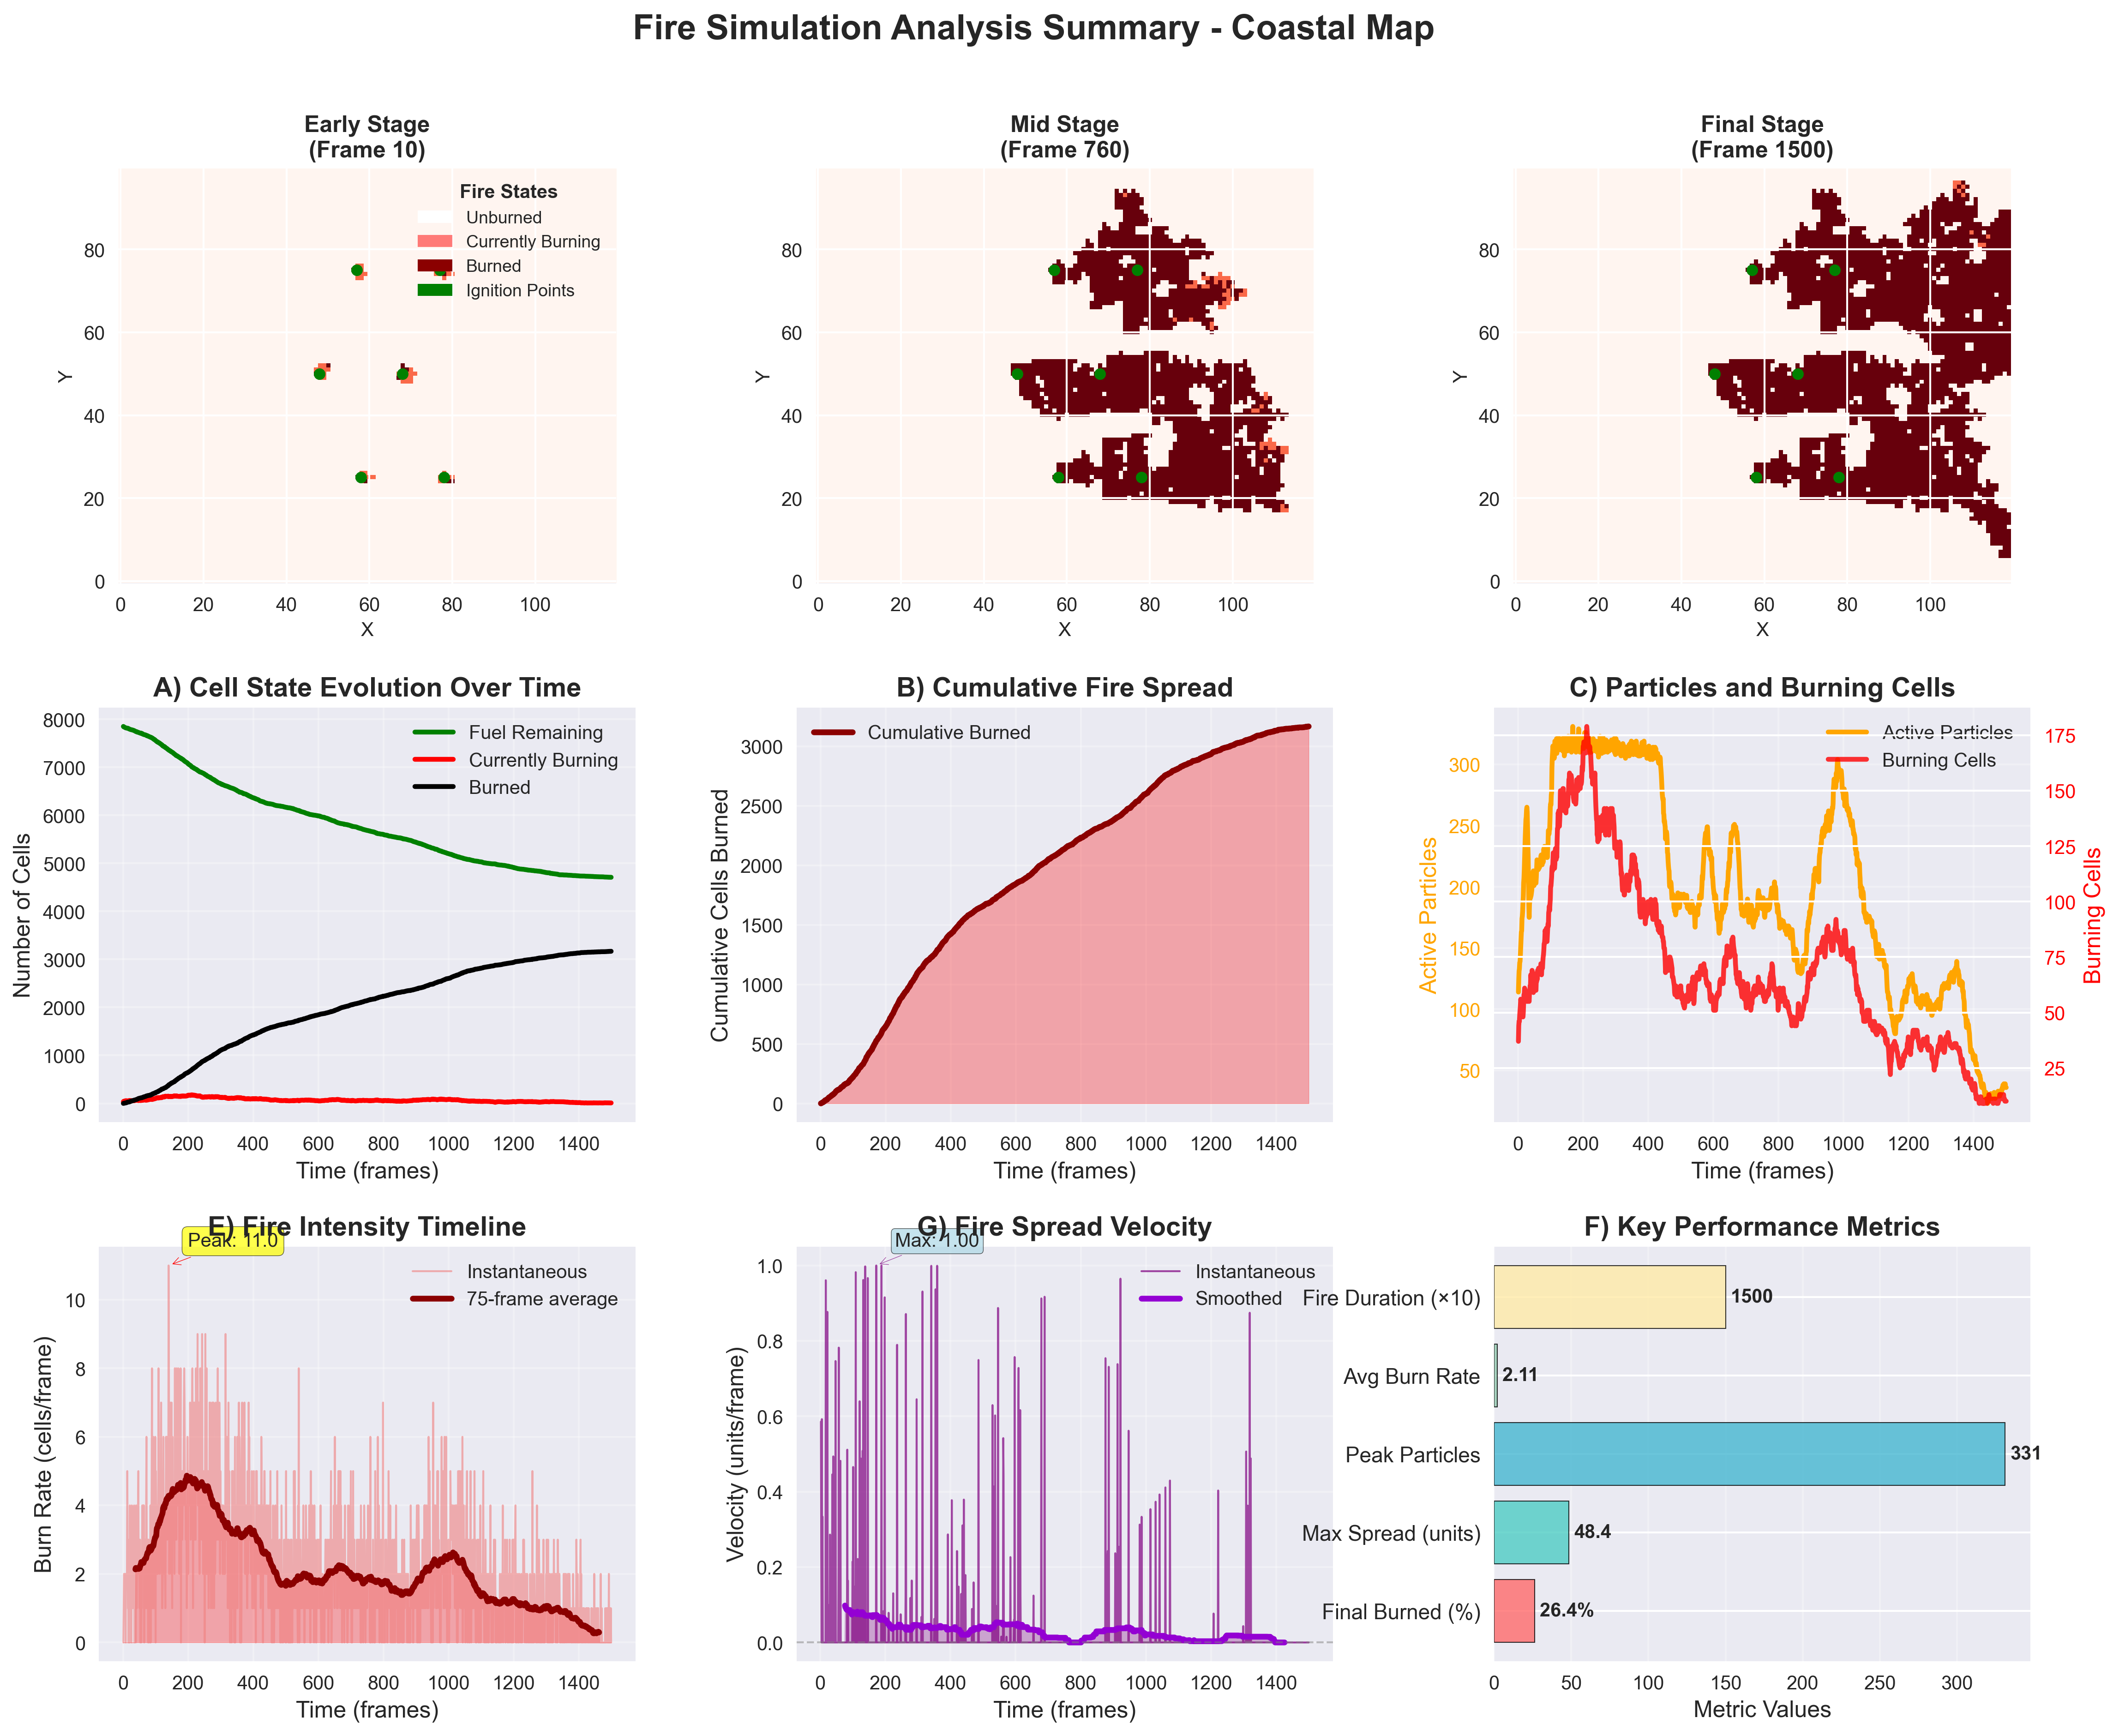
\includegraphics[width=\textwidth]{media/report_summary_coast.png}
	\caption{
		\textbf{Fire Simulation Analysis Summary - Coastal Fire Scenario.} 
		Analysis of coastal fire dynamics under strong offshore wind conditions with natural moisture barriers. Top row shows fire progression from multiple coastal ignition points (left) through inland advancement (center) to final contained burn pattern (right). The analysis demonstrates the protective effect of coastal moisture gradients, resulting in 28.4\% final burned area - the lowest of all scenarios - while showing characteristic wind-driven inland fire advancement with natural coastal barriers providing effective fire suppression.
	}
	\label{fig:res_coast}
\end{figure}
